\documentclass[10pt,landscape]{article}
\usepackage{multicol}
\usepackage{calc}
\usepackage{amsmath,amsthm,amsfonts,amssymb,relsize}
\usepackage{color,graphicx,overpic}
\usepackage{enumitem}
\usepackage{bm}
% \usepackage[landscape]{geometry}
\usepackage{algorithm}
\usepackage{algpseudocode}

\usepackage[cheatsheet]{preamble}
\definecolor{MyRoyalBlue}{RGB}{65,105,225} % RGB for Royal Blue
\definecolor{SubsectionGreen}{RGB}{180, 175, 80} % A soft green
% Turn off header and footer
\pagestyle{empty}
\geometry{top=.25in,left=.25in,right=.25in,bottom=.25in}


\definecolor{MyRoyalBlue}{RGB}{65,105,225} % RGB for Royal Blue
\definecolor{SubsectionGreen}{RGB}{75, 175, 80} % A soft green

% Redefine section commands to use less space
\makeatletter
\renewcommand{\section}{\@startsection{section}{1}{\z@}{3ex}{2ex}
                       {\normalfont\normalsize\bfseries\color{MyRoyalBlue}\textit}}
\renewcommand{\subsection}{\@startsection{subsection}{2}{\z@}{2ex}{0.5ex}
                          {\normalfont\small\bfseries\color{SubsectionGreen}}}
\renewcommand{\subsubsection}{\@startsection{subsubsection}{3}{0mm}%
                          {-1ex plus -.5ex minus -.2ex}%
                          {1ex plus .2ex}%
                          {\normalfont\small\bfseries}}
\makeatother

\setlist[itemize]{label={}, leftmargin=*, topsep=0pt, parsep=0.5pt, partopsep=0pt} % Remove margins from lists. 

% Don't print section numbers
\setcounter{secnumdepth}{0}

\setlength{\parindent}{0pt}
\setlength{\parskip}{0pt}

\newcommand{\R}{\mathbb{R}}
\newcommand{\E}{\mathbb{E}}

\newcommand{\bb}{\mathbf{b}}
\newcommand{\bv}{\mathbf{v}}
\newcommand{\bx}{\mathbf{x}}
\newcommand{\by}{\mathbf{y}}
\newcommand{\bz}{\mathbf{z}}

\newcommand{\bA}{\mathbf{A}}
\newcommand{\bB}{\mathbf{B}}
\newcommand{\bH}{\mathbf{H}}
\newcommand{\bI}{\mathbf{I}}
\newcommand{\bJ}{\mathbf{J}}
\newcommand{\bX}{\mathbf{X}}
\newcommand{\bY}{\mathbf{Y}}
\newcommand{\bZ}{\mathbf{Z}}

\newcommand{\balpha}{\boldsymbol{\alpha}}
\newcommand{\bbeta}{\boldsymbol{\beta}}
\newcommand{\btheta}{\boldsymbol{\theta}}
\newcommand{\bmu}{\boldsymbol{\mu}}
\newcommand{\bxi}{\boldsymbol{\xi}}
\newcommand{\bSigma}{\boldsymbol{\Sigma}}
\newcommand{\bLambda}{\boldsymbol{\Lambda}}

\newcommand{\diag}{\text{diag}}
\newcommand{\tp}[1]{#1^{\prime}}
\newcommand{\inv}[1]{#1^{-1}}
\newcommand{\norm}[1]{\|#1\|}
\newcommand{\gaussian}[2]{\mathcal{N}(#1, #2)}
\newcommand{\inR}[2]{#1 \in \R^{#2}}


\newcommand{\ruler}{\\\noindent\rule{\linewidth}{0.25pt}\\}

% -----------------------------------------------------------------------
\begin{document}
\raggedright%
\footnotesize
\begin{multicols*}{3}
    % multicol parameters
    % These lengths are set only within the two main columns
    % \setlength{\columnseprule}{0.1pt}
    \setlength{\premulticols}{1pt}
    \setlength{\postmulticols}{1pt}
    \setlength{\multicolsep}{1pt}
    \setlength{\columnsep}{0pt}

    \section{Math Review}
    \begin{itemize}
        \item $\mat{X}$ and $\bY$ are \textbf{independent} iff $\Pr(\mat{X},\bY)=\Pr(\mat{X})\Pr(\bY)$
        \item $\mat{X}$ and $\bY$ are \textbf{uncorrelated} iff $\E(\mat{X},\bY)=\E(\mat{X})\E(\bY)$
        \item \underline{Expected} value of $g(X)$: \( E[g(X)] = \int_{-\infty}^{\infty}g(x)f(x) dx\)
        \item \underline{Variance} \( \sigma^2 = E[{(X - \mu)}^2] = E[X^2] - \mu^2\)
        \item Determinant of matrix is product of its eigenvalues.
    \end{itemize}
    $
        f(\va{x}) = \mat{A}\va{x} + \va{x}^{\top}\mat{A} + \va{x}^{\top}\va{x} + \va{x}^{\top}\mat{A}\va{x} \Rightarrow
        \frac{df(\va{x})}{d\va{x}} = \mat{A}^{\top} + \mat{A} + 2\va{x} + \mat{A}\va{x} + \mat{A}^{\top}\va{x}
    $
    \begin{align*}
        \nabla_{\va{x}} (\va{y} \cdot \va{z}) & = (\nabla_{\va{x}}) \va{z} + (\nabla_{\va{x}}) \va{y} & \nabla_{\va{x}} f(\va{y}) & = (\nabla_{\va{x}} \va{y}) (\nabla_{\va{y}} f(\va{y})) \\
        \nabla_w w^T Aw                       & = (A + A^T)w                                          & \mat{H}_{i,j}             & = \frac{\partial^2 f}{\partial x_i \partial x_j}
    \end{align*}
    \section{Perceptron (Lecture 2)}
    $f(\va{x}) = \va{w} \cdot \va{x} + \alpha = \sum_{i=1}^{d}w_i x_i + \alpha$,


    \textbf{Goal: } find $w$ s.t all constraints $y_i X_i \cdot w \ge 0$. Define a risk function and optimize it, where the loss is defined as $L(z, y_i) = -y_i z \;\text{  if } y_i z < 0, \;\text{else }0$. Therefore risk $R(w) = \sum_{i \in V}-y_i X_i \cdot w$
    \ruler%
    \textbf{Decision boundary}, a \textbf{hyperplane} in $\R^d$: $H = \{\inR{\va{x}}{d} : f(\va{x}) = 0\} = \{\inR{\va{x}}{d} : \va{w} \cdot \va{x} + \alpha = 0\}$
    \ruler%
    $\va{w}$ is the \textbf{normal} of the hyperplane,\\
    $\alpha$ is the \textbf{offset} of the hyperplane from origin,\\
    $\frac{f(\va{x})}{\norm{\va{w}}}$ is the \textbf{signed distance} from the \( \va{x} \) to hyperplane \( \mathcal{H} \).
    \ruler%
    \textbf{Perceptron algorithm},\\
    Input: $(\bx_1, y_1),\dots,(\bx_n, y_n) \in \R^{d} \times \{\pm 1\}$\\
    while some $y_i \neq \text{sign}(\va{w} \cdot \bx_i)$\\
    \-\hspace{0.5cm} pick some misclassified $(\bx_i, y_i)$\\
    \-\hspace{0.5cm} $\va{w} \leftarrow \va{w} + y_i\bx_i$
    \ruler%
    Given a \textbf{linearly separable data}, perceptron algorithm will take no more than $\frac{R^2}{\gamma^2}$ updates to \textbf{converge},
    where $R = \max_{i}{\norm{\bx_i}}$ is the radius of the data, $\gamma = \min_{i}{\frac{y_i(\va{w}\cdot\bx_i)}{\norm{\va{w}}}}$ is the margin.\\
    Also, $\frac{\va{w}\cdot\va{x}}{\norm{\va{w}}}$ is the signed distance from H to $\va{x}$ in the direction $\va{w}$.
    \ruler%
    \textbf{Gradient descent} view of perceptron, minimize margin cost function
    $J(\va{w}) = \sum_{i}{}{(-y_i(\va{w}\cdot\bx_i))}_{+}$ with $\va{w} \leftarrow \va{w} - \eta\nabla J(\va{w})$
    % --------------------------------

    \section{Support Vector Machine (Lecture 3, 4)}
    \textbf{Hard margin SVM},\\
    This method makes the margin as wide as possible.
    The signed distance from the hyperplane to $X_i$ is$\frac{f(\bx_i)}{\lVert w \rVert}$
    Hence the margin is $\min_i \frac{1}{\lVert w \rVert} |w \cdot X_i + \alpha|  \ge \frac{1}{\lVert w \rVert} \implies$
    $\min_{\va{w}} \norm{\va{w}}^2$, such that $y_i\va{w}\cdot\bx_i \geq 1 (i = 1,\dots,n)$\\
    \textbf{Soft margin SVM},\\
    $\min_{\va{w}} \norm{\va{w}}^2 + C\sum_{i = 1}^{n} \xi_i$
    \ruler%
    \textbf{Regularization and SVMs}:
    Simulated data with many features $\phi(\va{x})$;
    C controls trade-off between margin $1/\norm{\va{w}}$ and fit to data;
    Large C\@: focus on fit to data (small margin is ok). More overfitting.
    Small C\@: focus on large margin, less tendency to overfit.
    Overfitting increases with: less data, more features.
    % --------------------------------
    \section{Decision Theory (Lecture 6)}
    \textbf{Bayes Theorem:} \( \underbrace{\Pr(Y = C | X)}_{\text{Poster. Prob}} = \frac{\Pr(X | Y = C) \overbrace{\Pr(Y = C)}^{\text{Prior Prob.}}}{\Pr(X)} \)
    Assume $(\mat{X}, \bY)$ are chosen i.i.d according to some probability distribution on $\mathcal{X}\times\mathcal{Y}$.
    \textbf{Risk} is misclassification probability: $R(r) = \E (L(r(\mat{X}), \bY)) = \Pr(r(\mat{X})
        \neq \bY) =$

    \( \sum_{\va{x}} \big[ L(r(\va{x}), 1)\Pr(Y = 1|x) + L(r(x), -1)\Pr(Y = -1|X = \va{x}) \big] \times \Pr(\va{x}) \)
    \ruler%
    \( = \Pr(Y = 1) \sum_x L(r(\va{x}), 1)\Pr(\va{x}|Y = 1) + \Pr(Y = -1) \sum_x L(r(\va{x}), -1)\Pr(\va{x}|Y = -1)\)
    \ruler%
    \textbf{Bayes Decision Rule} is
    $
        r^{*}(x) =
        \begin{cases}
            1,  & \text{if } L(-1, 1)\Pr(\bY=1|x) > L(1, -1)\Pr(\bY=-1|x) \\
            -1, & \text{otherwise. }
        \end{cases}
    $,\\
    and the optimal risk (Bayes risk) $R^{*} = \inf_{r}R(r)=R(r^*)$
    % --------------------------------

    \section{Generative and Discriminative Models (Lecture 6)}
    \textbf{Discriminative models}: $\Pr(\mat{X}, \bY) = \Pr(\mat{X})\Pr(\bY|\mat{X})$.\\
    Estimate $\Pr(\bY|\mat{X})$, then pretend our estimate $\hat{\Pr}(\bY|\mat{X})$ is the actual $\Pr(\bY|\mat{X})$ and
    plug in bayes rule expression.
    \ruler%
    \textbf{Generative model}: $\Pr(\mat{X}, \bY) = \Pr(\bY)\Pr(\mat{X}|\bY)$.\\
    Estimate $\Pr(\bY)$ and $\Pr(\mat{X}|\bY)$, then use bayes theorem to calculate $\Pr(\bY|\mat{X})$ and use discriminative model.
    \ruler%
    \textbf{Gaussian} class conditional densities $\Pr(\mat{X}|Y=+1)$,$\Pr(\mat{X}|Y=-1)$ (with the same variance), the posterior probability is \textbf{logistic}:\\
    $\Pr(Y=+1|\va{x}) = \frac{1}{1+\text{exp}(-\va{x}\cdot\va{w}-\beta_0)}$,\\
    $\va{w} = \inv{\Sigma}(\bmu_{1}-\bmu_{0})$, $\beta_0=\frac{\tp{\bmu_{0}}\inv{\Sigma}\bmu0-\bmu_{1}\inv{\Sigma}\bmu1}{2}+\log\frac{\Pr(Y=1)}{\Pr(Y=0)}$
    % --------------------------------

    \section{Multivariate Normal Distribution (Lecture 7)}
    $\inR{\va{x}}{d}: p(x) = \frac{1}{{(2\pi)}^{d/2}|\bSigma|^{1/2}}e^{(-\frac{1}{2}\tp{(\va{x}-\bmu)}\inv{\bSigma}(\va{x}-\bmu))}$
    \ruler%
    \textbf{QDA:} Class-conditional densities \( X_C \sim \gaussian{\va{\mu}_C}{\Sigma_C}\). Optimal decision rule \( r^*(x) \) for 0--1 loss: Choose class \textbf{C} that maxes \( \Pr(Y = C|X) \propto f_C(x)\pi_C \). Parameters estimated via MLE\@:

    \textbf{LDA:} Assumes equal covariance matrices across classes (\( \Sigma_C = \Sigma \)), simplifying to linear decision surfaces.
    \ruler%
    $\bSigma = \E(\mat{X} - \bmu)\tp{(\mat{X} - \bmu)}$\\
    Symmetric: $\bSigma_{i,j} = \bSigma_{j_i}$\\
    Non-negative diagonal entries: $\bSigma{i,i} \geq 0$\\
    Positive semidefinite: $\forall \inR{\bv}{d}, \tp{\bv}\bSigma\bv \geq 0$
    \ruler%
    Given a $d$-dimensaional Gaussian $\mat{X} \sim \gaussian{\bmu}{\bSigma}$,\\
    matrix $\inR{\mat{A}}{m\times d}$ and vector $\inR{\bb}{m}$, define $\bY = \mat{A}\mat{X} + \bb$.\\
    Then $\bY \sim \gaussian{\mat{A}\bmu + \bb}{\mat{A}\bSigma\mat{A}^{\top}}$
    \ruler%
    Given a $d$-dimensaional Gaussian $\mat{X} \sim \gaussian{\bmu}{\bSigma}$,\\
    with $\bSigma$ positive definite,\\
    $\bY = \bSigma^{-\frac{1}{2}}(\mat{X}-\bmu) \sim \gaussian{\va{0}, \bI}$
    \ruler%
    \subsection{MLE's}
    \textbf{Maximum a posterior probability}: the mode of the posterior. If uniform prior, MAP is MLE; if not
    uniform prior, MAP is Penalized MLE.
    % --------------------------------

    \begin{itemize}
        \item \textbf{Prior:} \( \hat{\pi}_C = \Pr(Y=C) = \frac{N_C}{n} \)
        \item \textbf{Mean:} \( \hat{\mu}_C = \E[\mat{X}|Y=C] = \frac{1}{N_C} \sum\limits_{i:Y_i = C} X_i \)
        \item \textbf{Covariance:} \( \hat{\Sigma}_C = \frac{1}{N_C} \sum\limits_{i:Y_i = C} (X_i - \hat{\mu}_C)(X_i - \hat{\mu}_C)^\top \)
        \item \textbf{Pooled Cov:} \( \hat{\Sigma} = \frac{1}{n} \sum\limits_{C_k} \sum\limits_{i:Y_i = C_k} (X_i - \hat{\mu}_{C_k})(X_i - \hat{\mu}_{C_k})^\top \)
    \end{itemize}
    \section{Discriminant Analysis (Lecture 7)}
    \textbf{Discriminant Functions for LDA and QDA} for class $C$, denoted \(Q_C(\va{x})\) is:
    \[
        Q_C(\va{x}) = \ln \left( \frac{f_{\va{X}|Y=C}(\va{x}) \pi_C}{(2\pi)^{\frac{d}{2}}} \right) = -\frac{1}{2}(\va{x} - \bm{\mu}_C)^T \bm{\Sigma}_C^{-1} (\va{x} - \bm{\mu}_C) - \frac{1}{2}\ln |\bm{\Sigma}_C| + \ln \frac{\pi_C}{(2\pi)^{\frac{d}{2}}}
    \]
    Here we have, the class-conditional density \(f_{\va{X}|Y=C}(\va{x})\), prior probability \(\pi_C\), the mean vector of class \(C\), and covariance matrix \(\bm{\Sigma}_C\) of class $C$.
    \ruler%
    \textbf{Linear Decision Function between Classes C and D:}
    Compares classes by:

    \[
        Q_C(\va{x}) - Q_D(\va{x}) = (\bm{\mu}_C - \bm{\mu}_D)^T \bm{\Sigma}^{-1} \va{x} - \frac{1}{2} (\bm{\mu}_C^T \bm{\Sigma}^{-1} \bm{\mu}_C - \bm{\mu}_D^T \bm{\Sigma}^{-1} \bm{\mu}_D) + \ln \frac{\pi_C}{\pi_D}.
    \]
    This expression includes a linear term \((\bm{\mu}_C - \bm{\mu}_D)^T \bm{\Sigma}^{-1} \va{x}\), which describes how the decision boundary is formed linearly in the feature space, and a constant term that adjusts the boundary based on the means of the classes and their prior probabilities.
    \ruler%
    \textbf{Multi-class LDA:}
    The optimal class for a given feature vector \(\va{x}\) is chosen by
    \[
        \text{Choose class } C \text{ such that } Q_C(\va{x}) \text{ is maximized.}
    \]
    Effectively determining the most likely class based on the feature measurements and statistical properties of each class.

    \section{Linear Regression (Lecture 10)}
    \textbf{Objective Function:}
    The goal in linear regression is to minimize the sum of squared residuals (RSS), expressed as:
    \[
        \text{RSS}(\va{w}) = \sum_{i=1}^{n} (\va{x}_i^\top \va{w} + \alpha - y_i)^2 = \norm{\mat{X}\va{w} - \va{y}}^2.
    \]
    Where, \(\mat{X} \in \R^{n \times (d + 1)}\) is the \textbf{design matrix}, and \(\va{y}\) is the \textbf{response vector}.

    \textbf{Minimize via Calculus:}
    \( \nabla \text{RSS}(\va{w}) = 2\mat{X}^\top \mat{X} \va{w} - 2\mat{X}^\top \va{y}. \)\\
    Setting this gradient to zero leads to the \textbf{normal equations}:
    \[
        \mat{X}^\top\mat{X}\va{w} = \mat{X}^\top\va{y},
    \]
    Solving for the optimal weights \(\va{w}^*\):
    \[
        \va{w}^* = (\mat{X}^\top\mat{X})^{-1}\mat{X}^\top\va{y},
    \]
    $(\mat{X}^\top\mat{X})^{-1}\mat{X}^\top$ is known as the \textit{Moore-Penrose pseudo-inverse} \(X^\dagger\) of \(\mat{X}\).

    \textbf{Projection Theorem} also leads to the normal equations, by asserting that the solution \(\va{w}^*\) projects the residuals orthogonally onto the column space of \(\mat{X}\):
    \[
        \mat{X}^\top (\va{y} - \mat{X}\va{w}) = 0 \implies \mat{X}^\top \mat{X}\va{w} = \mat{X}^\top \va{y},
    \]
    % --------------------------------


    \section{Logistic Regression (Lecture 10, 11)}
    Fits ``probabilities'' to data and usually used for classification.
    $\Pr(Y=1|\va{x}_i)=\frac{1}{1+\text{exp}(-\va{w}^{\top}\va{x}_i)} = \sigma(\va{w}^{\top}\va{x}_i)$

    \textbf{Logistic Loss:} $L(z, y) = -y\ln z - (1 - y)\ln(1 - z)$\\
    \textbf{Cost Function:} $J(\va{w}) = - \sum_{i = 1}^{n} L\left(\sigma(\va{w}^{\top}\va{x}_i), y_i\right)$\\
    Find $\va{w}^* = \arg \min J(\va{w})\;\;\;$, Cost function is convex, and solved by gradient descent. Converges to max margin classifier.
    \ruler%
    Let $\sigma_i = \sigma(\va{w}^{\top}\va{x}_i)$ and $\va{\sigma} = \begin{bmatrix}
            \sigma_1 & \cdots & \sigma_n
        \end{bmatrix}^\top$
    \begin{itemize}
        \item $\nabla_{\va{w}} \sigma_i = \sigma_i(1 - \sigma_i)\va{x}_i$
        \item $\nabla_{\va{w}} J(\va{w}) = \mat{X}^{\top}(\va{\sigma} - \va{y})$
        \item $\nabla_{\va{w}}^2 J(\va{w}) = \mat{X}^{\top}\diag\left(\va{\sigma}(1-\va{\sigma})\right)\mat{X}$
    \end{itemize}
    \textbf{Gradient descent}:\\
    $\va{w}^{(t+1)}=\va{w}^{(t)} - \eta\nabla_{\va{w}}J(\va{w}^{(t)})$ : $O(nd)$ per step\\
    \textbf{Stochastic gradient descent}:\\
    $\va{w}^{(t+1)}=\va{w}^{(t)} - \eta \nabla L_i (\va{w}^{(t)})$ : $O(d)$ per step\\
    \textbf{Newton's method}:\\
    $\va{w}^{(t+1)}=\va{w}^{(t)} - \inv{\left(\nabla^2 J(\va{w}^{(t)})\right)}\nabla J(\va{w}^{(t)})$
    \ruler%
    \subsection{LDA vs. Logistic Regression}
    \textbf{Advantages of LDA:}
    \begin{itemize}[label=\textbullet]
        \item For well-separated classes, LDA is stable; log\@. reg\@. is suprisingly unstable.
        \item > 2 classes? Easy \& elegant; log\@. reg\@. needs modifying\@. (softmax regr.)
        \item slightly more accurate when classes nearly normal, especially if $n$ is small.
    \end{itemize}
    \textbf{Advantages of Log. Regression:}
    \begin{itemize}
        \item More emphasis on desc\@. boundary; always separates linearly separable pts.
        \item More robust on some non-Gaussian distributions (e.g., dists w/ large skews.)
        \item Naturally fits labels between $0$ and $1$.
    \end{itemize}

    \subsection{ROC CURVES}
    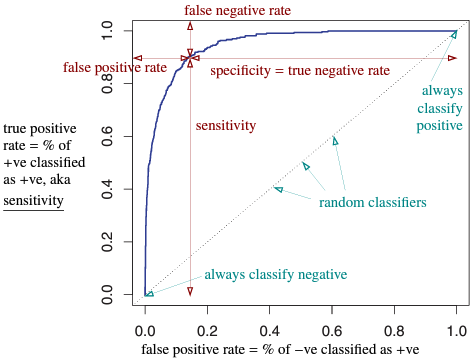
\includegraphics[scale=0.5]{./images/ROC-curve.png}
    \ruler%TODO Remove

    \section{Polynomial Regression (Lecture 11)}
    Replace each $x_i$ with feature vector $\Phi(x_i)$ with all terms of degree $p$ polynomial.
    e.g.,$ \Phi(x_i) = \begin{bmatrix} x^2_{i1} & x_{i1}x_{i2} & x^2_{i2} & x_{i1} & x_{i2} &  1 \end{bmatrix}^\top$
    \ruler%
    Log. Reg. + quadratic features = same form of posteriors as QDA\@.

    \section{Statistical Justification For Regression (Lecture 12)}
    Typical model of reality:
    $\forall X_i, \, y_i = g(X_i) + \epsilon_i\,\,$: $\epsilon_i \sim D^\prime$ where $D^\prime$ has mean 0.

    Ideal approach: choose $h(X_i) = \E_y[Y | X = X_i] = g(X_i) + \E[\epsilon_i] = g(X_i)$
    \subsection{Least Squares Cost Function From MLE}
    Suppose $\epsilon_i \sim \Norm\left(0, \sigma^2\right) \implies y_i \sim \Norm\left(g(\va{x}_i), \sigma^2\right)$. We're going to try to estimate $g(\va{x})$, which is defined by some weights $\va{w}$. The probability of $y_i$, given it's parameters for its distribution, is a pdf $f(y_i)$ \& the log likelihood is:
    \begin{align*}
        \ell(g; \mat{X}, \va{y}) & = \ln(\prod_{i=1}^n f(y_i))
        = \sum_{i = 1}^{n} \ln(f(y_i))
        = -\frac{1}{2\sigma^2}\sum_{i = 1}^{n}\left(y_i - g(\va{x}_i)\right)^2 - C
    \end{align*}
    Maximumizing this is equivalent to minimizing $\sum_{i = 1}^{n}\left(y_i - g(\va{x}_i)\right)^2 = \text{RSS}$

    \subsection{Logistic Loss from MLE}
    Consider $P[\va{x}_i \in \text{class C}] = y_i$ as the actual probability, with $h(\va{x}_i)$ as the predicted probability. For $\beta$ hypothetical repetitions, where $y_i\beta$ samples belong to class C and $(1 - y_i)\beta$ do not. The likelihood of $h$ given the data is:
    \[
        \mathscr{L}(h; \mat{X}, \va{y}) = \prod_{i = 1}^{n} h(\va{x}_i)^{y_i \beta} (1 - h(\va{x}_i))^{(1 - y_i)\beta}
    \]
    \[
        \ell(h; \mat{X}, \va{y}) = \beta \sum_{i = 1}^{n} \left[ y_i \ln (h(\va{x}_i)) + (1 - y_i) \ln (1 - h(\va{x}_i)) \right]
    \]
    Maximizing the log likelihood $\ell(h)$ is equivalent to minimizing logistic losses.

    \subsection{The Bias-Variance Decomposition}
    There are 2 sources of error in a hypothesis $h$:
    \begin{itemize}
        \item \textbf{bias}: error due to inability of hypothesis $h$ to fit $g$ perfectly.
        \item \textbf{variance}: error due to fitting random noise in data, e.g., we fit linear $g$ with a linear $h$, yet $h \neq g$.
    \end{itemize}

    Model: $X_i \sim D$, $\epsilon_i \sim D^\prime$ and $y_i = g(X_i) + \epsilon_i$. Fit hypothesis $h$ to $\mat{X}, \va{y}$. Now $h$ is a r.v., because of the random noise $\epsilon$. Let $z$ be an arbitrary pt and $\gamma = g(z) + \epsilon$
    Now the risk fn when loss is the squared errror is:\\
    $R(h) = \E[L(h(z), \gamma)] \leftarrowtail$ exp over possible training set $X, y$ and values of $\gamma$\\
    $R(h) = \E[(h(z) - \gamma)^2]$\\
    $R(h) = \E[h(z)^2] + \E[\gamma^2] - 2\E[\gamma h(z)]$\\
    $R(h) = \Var(h(z)) + {\E[h(z)]}^2 + \Var(\gamma) + {\E[\gamma]}^2 - 2\E[\gamma] \E[h(z)]$\\
    $R(h) = \left(\E[h(z)] - \E[\gamma]\right)^2 + \Var(h(z)) + \Var(\gamma)$\\
    $R(h) = \underbrace{\left(\E[h(z)] - \E[\gamma]\right)^2}_{\text{bias}^2 \text{ of method}} + \underbrace{\Var(h(z))}_{\text{variance of method}} + \underbrace{\Var(\epsilon)}_{\text{irreducible error}}$\\
    \begin{itemize}[label=$\bullet$]
        \item \textbf{Underfitting}: Too much bias
        \item \textbf{Overfitting}: Too much variance
        \item Training Error reflects bias but not variance
        \item Test error reflects both.
    \end{itemize}

    \section{Linear Regression Regularization (Lecture 13)}
    \textbf{Trading off bias/variance}: some increase in bias can give big decrease in var.
    \ruler%
    \textbf{Ridge regression} is like $L2$ regularization: \\
    $\hat{\va{w}} = \text{arg }\min_{\va{w}}\norm{\va{y} - \mat{X}\va{w}}^2 + \lambda \norm{\va{w}}^2$, for some cost function $J$ on classifier $h$\\
    Minimized w/ Calculus\\
    $\hat{\va{w}}^{\text{ridge}}=\inv{(\mat{X}^{\top}\mat{X}+\lambda\bI)}\va{x}^{\top}\va{y}$
    \ruler%
    \textbf{Lasso regression} is like $L1$ regularization:\\
    $\hat{\va{w}} = \text{arg }\min_{\va{w}}\norm{\va{y} - \mat{X}\va{w}}^2 + \lambda \norm{w}_1$\\
    Minimized w/ Calculus (it's also a quadratic program)\\
    While ridge regression leads to reduced, but rare non-zero values of the weights,
    Lasso regression forces some weights to be zero.
    \ruler%
    \textbf{Bayesian analysis}:
    Ridge regression is equivalent to a MAP estimate with a gaussian prior.
    Lasso regression is equivalent to a MAP estimate with a Laplace prior.
    % --------------------------------
    \section*{Misc}
    \begin{itemize}
        \item \textbf{Centering} $\mat{X}$: This involves subtracting $\bm{\mu}^T$ from each row of $\mat{X}$. Symbolically, $\mat{X}$ transforms into $\bar{\mat{X}}$.
        \item \textbf{Decorrelating} $\mat{X}$: This process applies a rotation $\mat{Z} = \bar{\mat{X}}\mathbf{V}$, where $\text{Var}(\mathbf{R}) = \mathbf{V\Lambda V}^T$. This step rotates the sample points to the eigenvector coordinate system.
        \item \textbf{Sphering:}  $\bar{\mat{X}}$: applying transform $\mat{W} = \bar{\mat{X}} \text{Var}(\mathbf{R})^{-\frac{1}{2}}$
        \item \textbf{whitening} \(\mat{X}\): centering + sphering, \(\mat{X} \rightarrow \mat{W}\)
    \end{itemize}

    \section{Decision Trees (Lecture 14)}
    Cuts x-space into rectangular cells, and works well with both categorical and quantitative features.

    Two types of nodes:
    \begin{enumerate}
        \item \textbf{internal}: test feature values \& branch accordingly
        \item \textbf{leaf}: they specify the class \( h(x) \)
              \ruler%
    \end{enumerate}
    \textbf{For classification} the learning algorithm is a greedy, top-down learning heuristic. Let S be subset of sample pts indices\\
    \textbf{Learning algorithm}\\
    % GrowTree(S)\\
    % \-\hspace*{0.5cm} if (\( y_i = C \) for all \( i \in S \) and some class \( C \)) \{\\
    % \-\hspace*{0.9cm} return new leaf(\( C \))\\
    % \-\hspace*{0.5cm} \} else \{\\
    % \-\hspace*{0.9cm} choose best splitting feature \( j \) and splitting value \( \beta \)\\
    % \-\hspace*{0.9cm} \( S_L = \lbrace i \in S: X_{ij} < \beta \rbrace \) \\
    % \-\hspace*{0.9cm} \( S_R = \lbrace i \in S: X_{ij} \ge \beta \rbrace \) \\
    % \-\hspace*{0.9cm} return new node(\( j, \beta, \) GrowTree(\( S_L \)), GrowTree(\( S_R \)))\\
    % \-\hspace*{0.5cm} \}

    \begin{algorithmic}
        \Function{GrowTree}{$S$}
        \If{all $y_i = C$ for all $i \in S$ and some class $C$}
        \State \Return \textit{new leaf}($C$)
        \Else
        \State Choose best splitting feature $j$ and splitting value $\beta$
        \State $S_L = \{ i \in S: X_{ij} < \beta \}$
        \State $S_R = \{ i \in S: X_{ij} \ge \beta \}$
        \State \Return \textit{new node}($j, \beta,$ \Call{GrowTree}{$S_L$}, GrowTree($S_R$))
        \EndIf
        \EndFunction
    \end{algorithmic}
\end{multicols*}
\end{document}
